\subsection{Desarrollo de aplicación completa}

El siguiente objetivo del trabajo fue desarrollar una aplicación completa que permitiese a los usuarios obtener los resultados de forma fácil. Esto fue decidido principalmente por dos razones:

\begin{itemize}
    \item Era necesario cumplir el requisito que afecta al nivel de conocimiento necesario para manejar la herramienta. Con una aplicación que tuviese interfaz gráfica, se podría manejar mucho mejor que 
    obligar al usuario a usar una consola de comandos o a conocer como funcionar las diferentes dependencias de las librerías usadas.
    \item Servía como oportunidad para mejorar los servicios que era capaz de proporcionar el sistema, además de poder diseñar la aplicación para poder aprovechar de forma eficiente los recursos del 
    \texttt{HardWare}.
\end{itemize}

Para desarrollar esta aplicación primero se seleccionó la librería de \acrfullr{gui}. Este paso fue importante porque existen muchas posibles librerías en el entorno de \texttt{Python}, pero cada una 
aporta diferentes utilidades y abstracciones, siendo las más comunes:
\begin{itemize}
    \item \texttt{TKinter}: es el \texttt{framework} más usado en \texttt{Python}. Es una librería simple y que no se suele usar para manejar datos multimedia, ya que es muy simple.
    \item \texttt{PyQT}: librería que internamente usa el \texttt{framework} \texttt{QT}. Es mucho más potente y capaz de manejar videos y elementos complejos.
    \item \texttt{Kivy}: librería pensada para el desarrollo de aplicaciones móviles.
    \item \texttt{PySimpleGUI}: es una librería \texttt{wrapper} sobre \texttt{Tkinter} y similares, por lo tanto es muy simple, pero limita mucho.
    \item \texttt{Remi}: se usa para crear interfaces web.
    \item \texttt{DearPyGUI}\cite{HoffstadtDearPyGuiDear}: librería muy reciente que se centra en dar al usuario la máxima eficiencia posible, usando aceleración \texttt{HardWare} a través de \texttt{OpenGL}.
\end{itemize}



Al estar trabajando con redes neuronales, queremos que la interfaz gráfica utilice la menor cantidad de recursos posible y de la manera más eficiente. Además, como se verá en los siguientes puntos, 
se implementaron partes multimedia en la aplicación, por lo tanto fue necesaria una librería centrada en la eficiencia, lo cual dejaba como posibles opciones 
\texttt{PyQT} y \texttt{DearPyGUI}, sin embargo por motivos personales del autor, la librería seleccionada fue \texttt{DearPyGUI}.

La selección se debe a la experiencia del autor en otros trabajos con la misma librería para realizar aplicaciones de manejo de cámaras IP. Al conocer ya la librería, se reducirían 
los posibles problemas y la necesidad de mirar documentación. Además de esta experiencia pasada, quedó patente que \texttt{DearPyGUI} es capaz de manejar los recursos del ordenador de forma muy eficiente.

\clearpage
\subsubsection{Diseño de interfaz para la aplicación}

Para realizar el diseño de la aplicación, se diseñó a través de la herramienta \texttt{DrawIO}, un esquema general del flujo y ventanas de la aplicación (completo en el \hyperref[esquema:FlujoVentanas]{anexo c}).\newline
Usando este esquema como idea general, se fue desarrollando la aplicación poco a poco, desde la ventana inicial hasta la ventana de datos

\begin{itemize}
    \item \textbf{Ventana inicial de la interfaz}: esta ventana tiene como objetivo que el usuario seleccione el video sobre el que quiere realizar la detección automática de movimiento, su aspecto se puede ver en la 
    \autoref{fig:InicialSinSeleccion}.
    \begin{figure}[H]
        \centering
        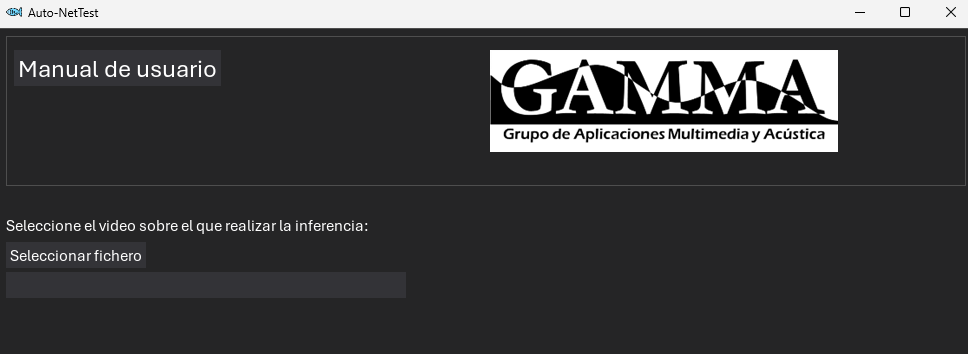
\includegraphics[width=0.9\textwidth]{images/6/6.5/VentanaInicial.png}
        \caption{Pantalla inicial sin video seleccionado}
        \label{fig:InicialSinSeleccion}
    \end{figure}

    Esta ventana contiene un botón que permite abril una ventana modal que contiene un manual de usuario. Esto se implementó para que las personas que usen esta aplicación no necesiten tener el documento de este trabajo a mano. 
    El aspecto de la ventana del manual se puede observar en la \autoref{fig:InicialManual}.

    \begin{figure}[H]
        \centering
        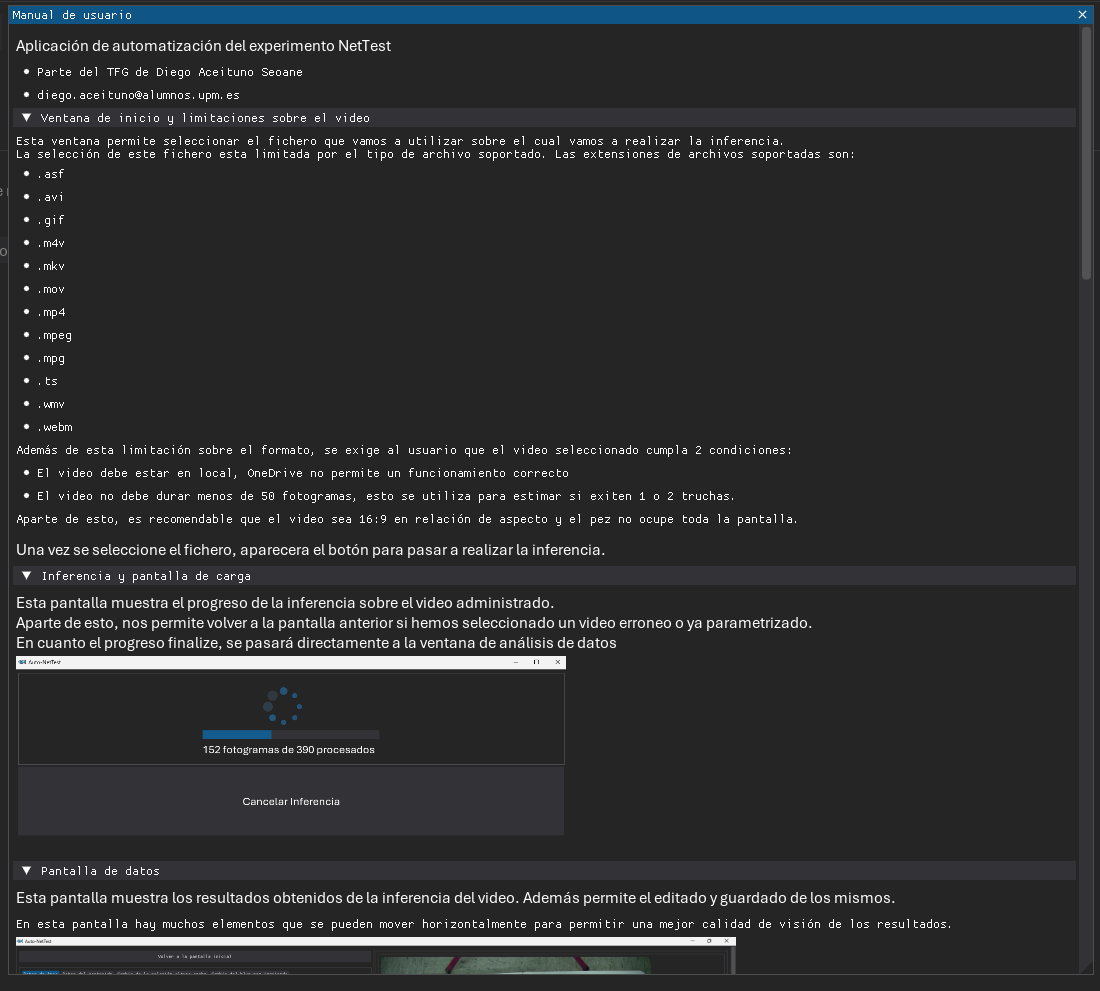
\includegraphics[width=0.8\textwidth]{images/6/6.5/Manual.png}
        \caption{Aspecto del manual contenido en la pantalla inicial de la aplicación}
        \label{fig:InicialManual}
    \end{figure}

    El usuario puede selecciona a través de un explorador de archivos, el fichero (debe ser un fichero soportado, lo cual se indica en el manual) sobre el que quiere realizar la inferencia. También puede utilizar el explorador 
    para cancelar la selección.
    
    En el momento que el fichero se selecciona, aparece un botón de inferencia como se ve en la \autoref{fig:InicialSeleccion}. Cuando se pulsa el botón, se realizan una series de comprobaciones sobre el video para ver sí es 
    compatible, en caso contrario la inferencia no se realizará y se volverá al estado inicial.

    \begin{figure}[H]
        \centering
        \begin{subfigure}{0.8\textwidth}
            \centering
            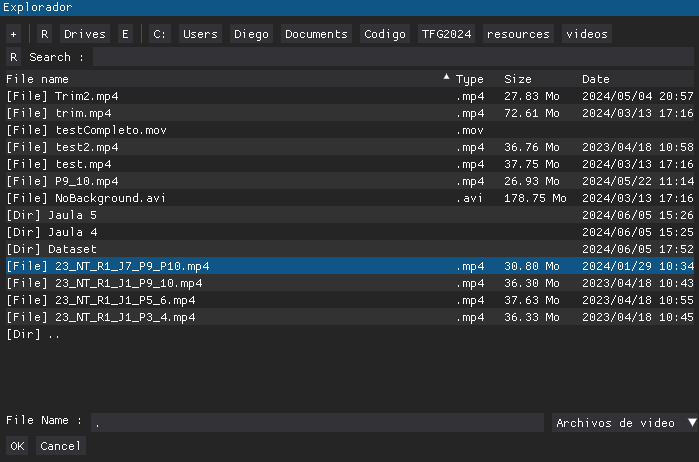
\includegraphics[width=0.9\textwidth]{images/6/6.5/Explorador.png}
            \caption{Aspecto del explorador de archivos para seleccionar video}
        \end{subfigure}
        \begin{subfigure}{0.8\textwidth}
            \centering
            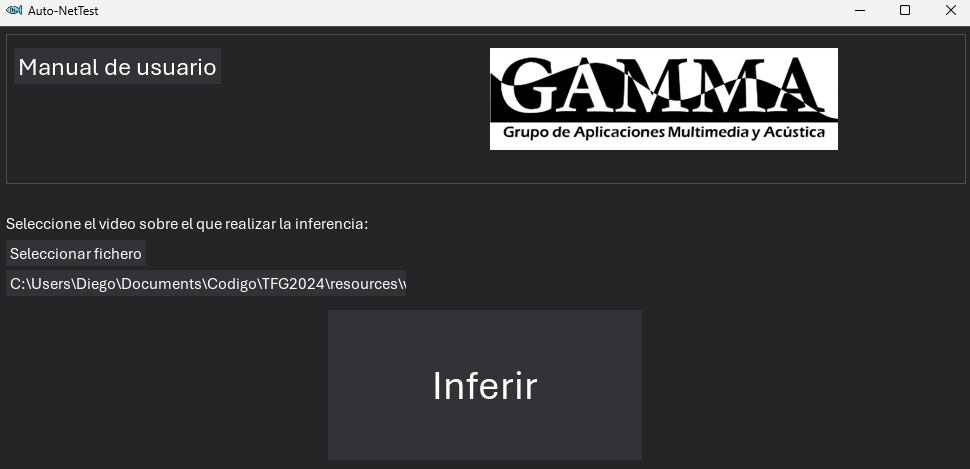
\includegraphics[width=0.9\textwidth]{images/6/6.5/InicialSeleccionado.png}
            \caption{En cuanto se selecciona el fichero, aparece el botón para iniciar el procesado}
        \end{subfigure}
        \caption{Flujo de selección de video}
        \label{fig:InicialSeleccion}
    \end{figure}
    \clearpage
    \item \textbf{Ventana de inferencia}: esta ventana sirve como pantalla de carga mientras se procesa el video, como se ve en la \autoref{fig:VentanaCarga} se implementó junto con un botón para cancelar por dos motivos:
    \begin{itemize}
        \item Permitir al usuario conocer el estado del procesamiento del video y que la aplicación no se quede estática.
        \item Permitir al usuario cancelar el proceso si se ha equivocado de video seleccionado.
    \end{itemize}
    \begin{figure}[H]
        \centering
        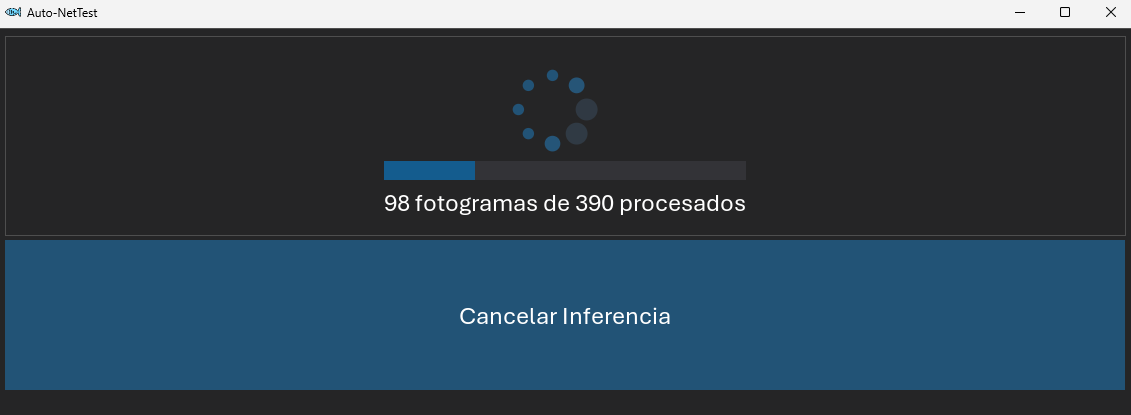
\includegraphics[width=0.8\textwidth]{images/6/6.5/Carga.png}
        \caption{Aspecto de la pantalla de carga de la aplicación}
        \label{fig:VentanaCarga}
    \end{figure}
\clearpage
    \item \textbf{Ventana de datos}: esta ventana tiene tres propósitos:
    \begin{itemize}
        \item Mostrar un análisis por gráficas sobre las \texttt{bounding boxes} de las truchas de cada lado, eliminando o añadiendo elementos de la \acrshort{gui} dependiendo de sí hay 1 o 2 truchas en el video. En concreto se 
        ha diseñado para mostrar 2 conjuntos de gráficas, el primer conjunto contiene gráficas para cada uno de los datos como el área, centroide, relación de tamaño y \texttt{blur} para las 2 truchas. El segundo conjunto tiene 
        una gráfica para cada trucha donde se representan la gráfica del área, centroide y \texttt{blur} al mismo tiempo.
        \item Mostrar el número de movimientos para cada trucha.
        \item Validar los resultados: se quería permitir que los usuarios pudiesen verificar los movimientos que han sucedido, para esto se han creado dos líneas de tiempo, una para cada trucha. A través de ellas y un reproductor 
        del video integrado en la aplicación, se pueden verificar los movimientos que han sucedido, pudiendo añadir o quitar movimientos.\newline
        Esta funcionalidad se realiza añadiendo la capacidad de que el usuario pueda pinchar en las líneas de tiempo, sirviendo como referencia del fotograma donde se quiere añadir el movimiento. Para que el usuario sepa donde está, se 
        marca con una línea vertical.
    \end{itemize}
    Los datos para rellenar las gráficas se obtienen cuando finaliza la inferencia previa y su transformación de datos, como se explicó en una sección anterior.\newline
    Elementos como las líneas de tiempo se han creado a base de unir gráficas y crear series discretas según los datos obtenidos. Estas series y gráficas se actualizan en tiempo de fotograma, además de ser ajustadas en altura 
    para aprovechar al máximo la pantalla del usuario y para no tener que depender de una aplicación a pantalla completa.

    El aspecto de esta ventana se puede verificar en la \autoref{fig:VentanaDatos}

    \begin{figure}[H]
        \centering
        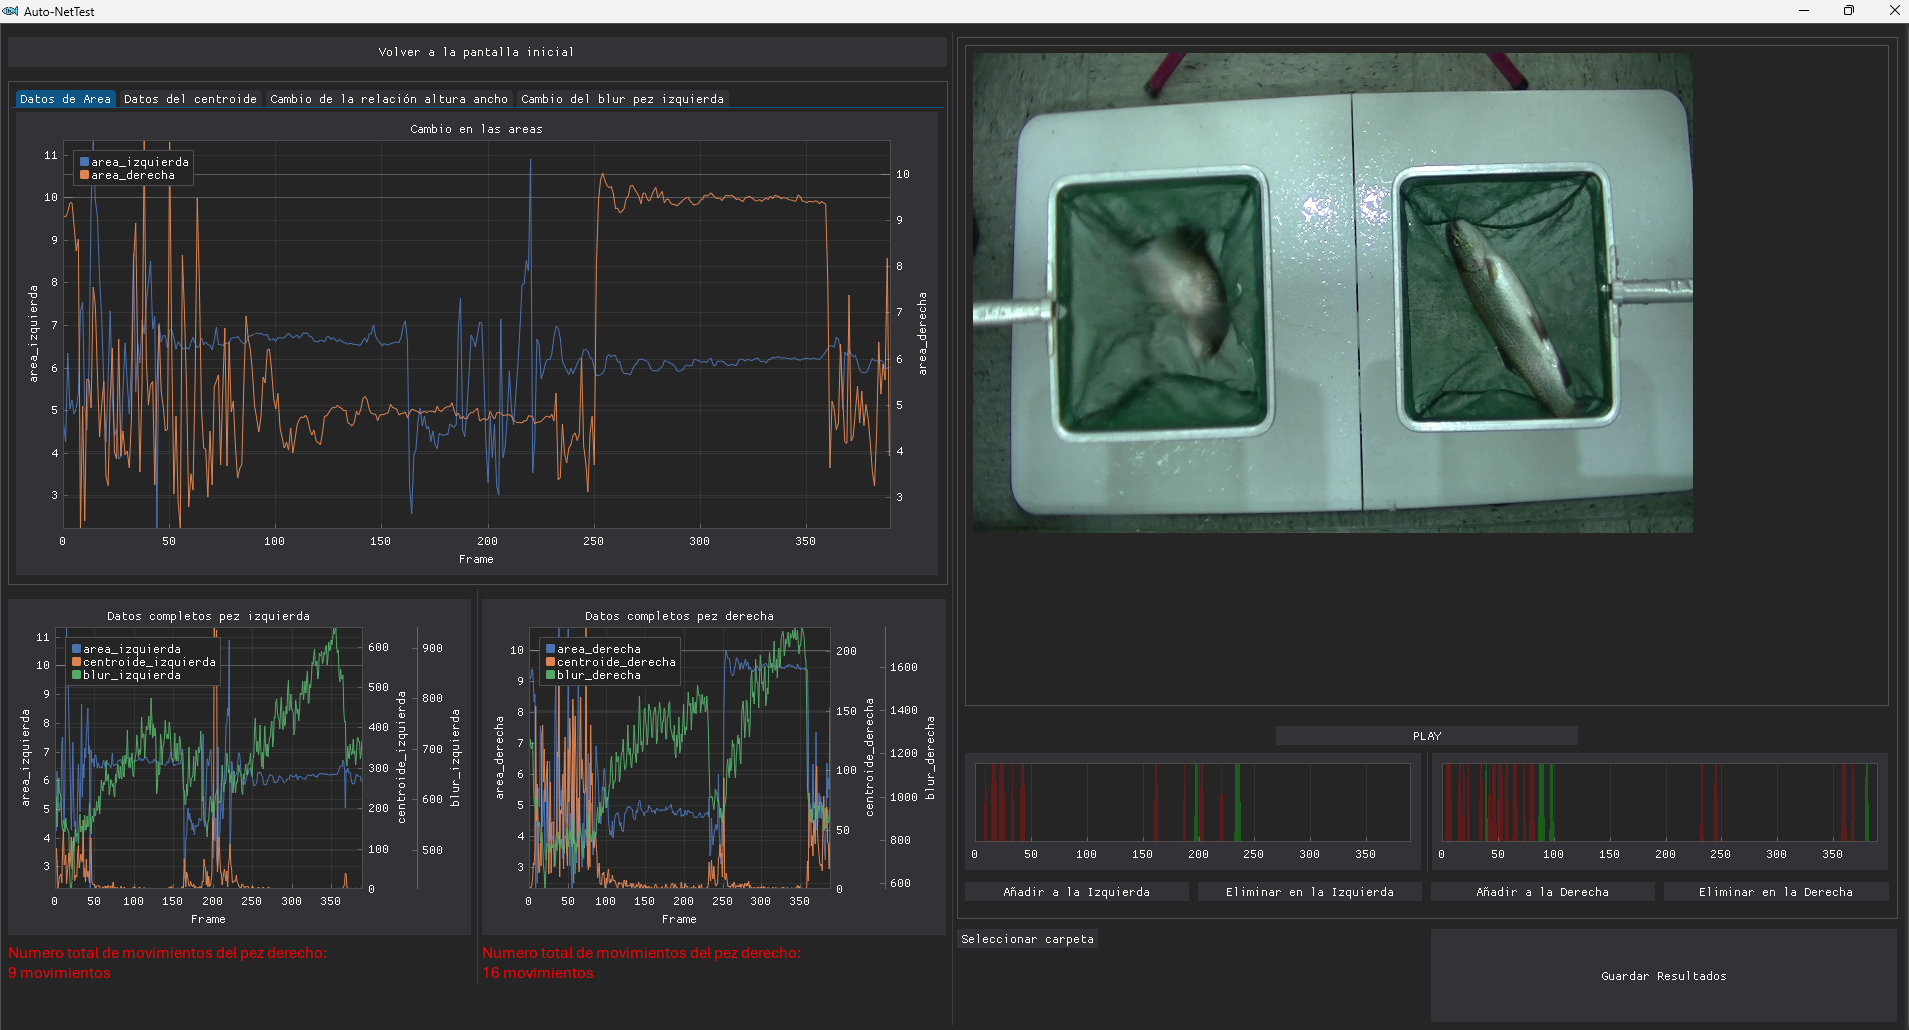
\includegraphics[width=0.95\textwidth]{images/6/6.5/VentanaDatos.png}
        \caption{Aspecto de la ventana de datos}
        \label{fig:VentanaDatos}
    \end{figure}
\end{itemize}
\clearpage
\subsubsection{Implementación de las funcionalidades a través de procesos}

Para poder implementar todas las funcionalidades de forma correcta, se necesitaba realizar de forma paralela diferentes tareas. Para esto se utilizó la librería \texttt{Multiprocessing} de \texttt{Python}.

El uso de \texttt{Multiprocessing} es debido a que la implementación de hilos en \texttt{Python} a través de la librería \texttt{Threading} no es como se espera. Esto es debido a que \texttt{Python} es 
un lenguaje interpretado, lo que implica que hay una aplicación que va analizando los ficheros de código y ejecutando operaciones.\newline
Para realizar esas tareas de forma segura respecto a la aplicación padre, \texttt{Python} implementa un \texttt{\acrfullr{gil}}, el cual evita que haya más de un hilo en ejecución a la vez.

Las implicaciones del \acrshort{gil} son en resumen:
\begin{itemize}
    \item El uso de hilos en \texttt{Python} se limita a situaciones especiales donde haya mucho \texttt{I/O}, ya que no son capaces de funcionar en paralelo.
    \item Para poder obtener concurrencia real, se necesita usar librerías que manejen varios intérpretes de \texttt{Python} a través de un lenguaje con mayor control como \texttt{C} o \texttt{C++}. 
    La librería \texttt{Multiprocessing} realiza esto, manejando los cambios de contexto y la relación entre procesos.
\end{itemize}

El uso de \texttt{multiprocessing}, al contrario que el uso de \texttt{threading} implica que no hay memoria compartida entre procesos, por lo tanto hay que pensar la forma para comunicar información 
entre procesos. Es un punto muy importante, ya que pueden aparecer problemas de concurrencia por falta de operaciones atómicas (1 línea de código de alto nivel no se ejecuta de golpe en el procesador).

Para la comunicación entre procesos existen muchas técnicas y sistemas ya existentes. En este trabajo se ha decidido utilizar técnicas basadas en colas. Aún sin ser el mecanismo que podría ser más 
eficiente en sobrecarga de memoria, es extremadamente fácil de usar.

Una cola es un mecanismo de bajo nivel que consiste en un \texttt{buffer} de tipo \texttt{\acrfullr{fifo}} que comunica diferentes procesos como se puede ver en la \autoref{fig:Pipe}. Permite operaciones de varios procesos productores y varios 
procesos consumidores. Además de esto, maneja los problemas de concurrencia de manera que el acceso para introducir y adquirir elementos se controle para todos los procesos, teniendo llamadas bloqueantes 
y métodos de \texttt{polling} sobre la cola.
\begin{figure}[H]
    \centering
    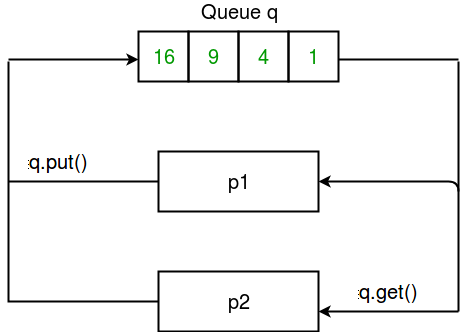
\includegraphics[width=0.5\textwidth]{images/6/6.5/Pipe.png}
    \caption{Funcionamiento de una cola para datos de procesos}
    \label{fig:Pipe}
\end{figure}

En la librería de \texttt{multiprocessing}, este mecanismo está completamente implementado de dos formas:
\begin{itemize}
    \item \texttt{Queue}: la cola que se ha explicado anteriormente, con varios productores y consumidores.
    \item \texttt{Pipe}: una cola que solo gestiona 1 productor y 1 consumidor. Es hasta 3 veces más rápida que una \texttt{Queue}, y por las tareas en las que se va a usar, es el mecanismo perfecto 
    para comunicar procesos en este trabajo. Cada objeto de esta clase cuenta con dos \texttt{enpoints}, uno para entrada de datos y otro para salida (si esto no se respeta saltan excepciones).
\end{itemize}
\clearpage
En este trabajo se utilizó \texttt{multiprocessing} para las siguientes tareas:
\begin{enumerate}
    \item \textbf{Realizar la inferencia}:\newline
    Cuando se creó una solución secuencial de prueba en anteriores secciones, se observó que procesar el \texttt{blur} de la imagen al final de procesar el video obligaba a acumular todas las imágenes 
    descomprimidas del video. Esto efectivamente creaba un pico en el uso de memoria \acrfullr{ram} (para un video de 15 s, era capaz de utilizar \texttt{3GB}), lo cual era extremadamente problemático.

    Para poder realizar la inferencia sin que la aplicación se quedase colgada y poder crear una pantalla de carga se implementó un sistema, en el que al momento de procesar un video, se crean dos procesos 
    en el programa principal a la vez que se crean dos objetos \texttt{Pipe}, comunicados como se ve en la \autoref{fig:DatosInferencia}:
    \begin{figure}[H]
        \centering
        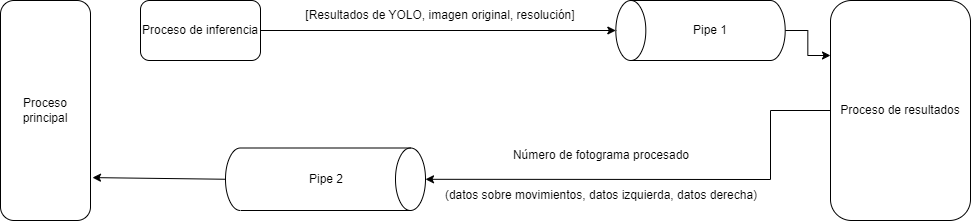
\includegraphics[width=0.9\textwidth]{images/6/6.5/Procesos1.png}
        \caption{Flujo de datos entre procesos para la inferencia}
        \label{fig:DatosInferencia}
    \end{figure}
    \vspace{2\baselineskip}
    \begin{itemize}
        \item Proceso de inferencia: va realizando la inferencia sobre el video fotograma a fotograma en modo streaming con el modelo \texttt{YOLO} entrenado en secciones anteriores. Antes de ser arrancado, 
        a este proceso se le pasa el \texttt{endpoint} que le permite introducir datos hacia el proceso para resultados. Para cada fotograma introduce en el \texttt{endpoint} un \texttt{array} que contiene: 
        [resultados del \texttt{YOLO}, imagen original, resolución de la imagen]. Para poder serializar correctamente los resultados de \texttt{YOLO} se utilizó la librería \texttt{Pickle} de \texttt{Python}.
        
        \item Proceso para resultados: este proceso va eliminando los mensajes que obtiene por el \texttt{endpoint} de salida en el que el proceso de inferencia va mandando los resultados y los acumula 
        en una variable propia. Cuando hay 50 mensajes, realiza la estimación del número de truchas que hay en el video, y a partir de aquí va procesando los resultados (incluyendo el cálculo del \texttt{blur}).
        Esto permite que las imágenes solo se guarden en memoria \texttt{RAM} el tiempo que estén en la \texttt{Pipe}. A la par que se realiza esto, a través del \texttt{endpoint} de entrada hacia el proceso 
        principal, se va indicando el fotograma por el que va el proceso de inferencia, lo cual permite rellenar la barra de carga para que el usuario pueda verlo. Cuando todos los resultados han sido 
        procesados, en el \texttt{endpoint} que se comunica con el proceso principal se manda un diccionario con el resultado del cálculo de movimientos y los datos de las truchas.
    \end{itemize}

    Una vez se ha acabado de procesar el video, se cambia de pantalla y se matan los anteriores procesos hijos creados.

    En el \hyperref[esquema:SecuenciaInferir]{anexo c} se puede encontrar un diagrama de secuencia con más detalle de estas operaciones.
    \clearpage
    \item \textbf{Mostrar el video en la pestaña de datos}:\newline
    Para permitir que el usuario pudiese editar los movimientos que han sucedido, se implementó una utilidad de reproducción de video. Esto se consigue añadiendo una textura a la interfaz y actualizándola 
    en cada bucle de renderizado. Para conseguir esto se implementó un proceso que controla la reproducción del video internamente manejando peticiones desde el hilo principal.
    Para esto se utilizan dos \texttt{Pipe}, uno del proceso principal al controlador de video, a través del cual se mandan indicaciones para comenzar la reproducción, parar y saltar a otra posición del video.\newline
    Estas comunicaciones se pueden ver en la \autoref{fig:DatosVideo}.

    Antes de entrar en la ventana de datos, se usa la primera imagen del video (esta se guardó al verificar los 50 fotogramas mínimos de duración antes de la pantalla de carga) para cargar en la textura.

    \begin{figure}[H]
        \centering
        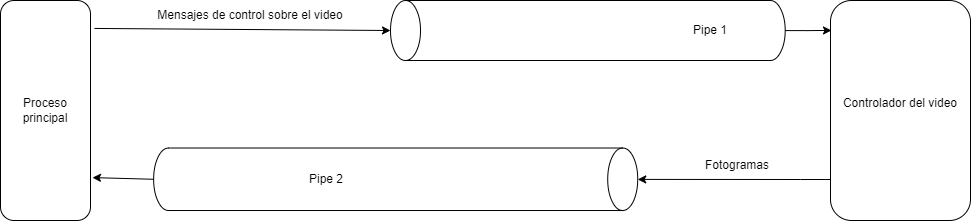
\includegraphics[width=0.9\textwidth]{images/6/6.5/Procesos2.png}
        \caption{Flujo de información entre el proceso principal y el controlador de video}
        \label{fig:DatosVideo}
    \end{figure}

    El proceso principal puede mandar como señales:
    \begin{itemize}
        \item True: indica que se debe reproducir el video para obtener fotogramas.
        \item False: indica que se debe pausar el video
        \item Un valor entero positivo: indica una posición en fotograma al que se debe saltar en el reproductor. Esta es la parte que permite al usuario verificar los diferentes movimientos.
    \end{itemize}
    El proceso controlador de video tomará como referencia temporal $ t = 0.8/fps $ y, sí se encuentra en modo reproducción, irá obteniendo, procesando y mandando los fotogramas en ese ritmo. Para todo 
    esto se aprovecha de la librería \texttt{OpenCV}.
    
    En el \hyperref[esquema:SecuenciaResto]{anexo c} se pueden encontrar los diagramas de secuencia que se asocian a estas situaciones.
\end{enumerate}

\vspace{2\baselineskip}

Aparte de todo lo anterior, se pueden encontrar todas las referencias de métodos, clases y módulos en el diagrama de clases general de la aplicación, el cual se encuentra en el 
\hyperref[esquema:DiagramaClases]{anexo c} de este documento.

\clearpage
\subsubsection{Guardado de los datos y despliegue de la aplicación}

Como parte del sistema global, se espera poder almacenar la información detectada en un fichero. Para realizar esto se añadió un selector de carpeta y un botón de guardado de resultados, como se puede 
ver en la \autoref{fig:Guardar}.

\begin{figure}[H]
    \centering
    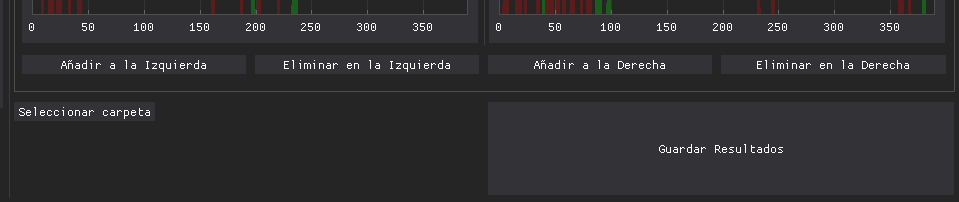
\includegraphics[width=0.8\textwidth]{images/6/6.5/Guardar.png}
    \caption{Widgets relacionados con el guardado}
    \label{fig:Guardar}
\end{figure}

Para permitir flexibilidad en el manejo de los datos, se guardan a la vez dos archivos:
\begin{itemize}
    \item Archivo \acrfullr{csv}: este tipo de archivos se pueden abrir directamente con editores de texto plano y son compatibles con Excel.\newline
    Manejan datos con un conjunto de separaciones por comas en horizontal, y saltos de líneas en vertical. En este caso se guarda la estructura de la \autoref{fig:CSVFormat}, no siendo obligatorio los datos 
    de la trucha de la derecha (esto ocurre cuando hay solo una trucha).
    \begin{figure}[H]
        \centering
        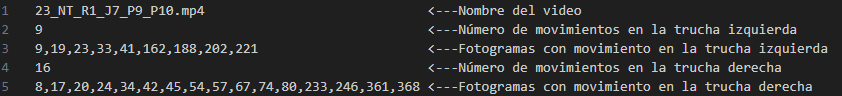
\includegraphics[width=0.9\textwidth]{images/6/6.5/csvFormat.png}
        \caption{Formato de los resultados guardados en \acrshort{csv}}
        \label{fig:CSVFormat}
    \end{figure}
    \item Archivo \acrfullr{json}: este tipo de archivos son semi-estructurados y funcionan muy bien, ya que se usan en todos los lenguajes de programación. En este caso la estructura que se guarda es 
    la de la \autoref{fig:JSONFormat}.
    \begin{figure}[H]
        \centering
        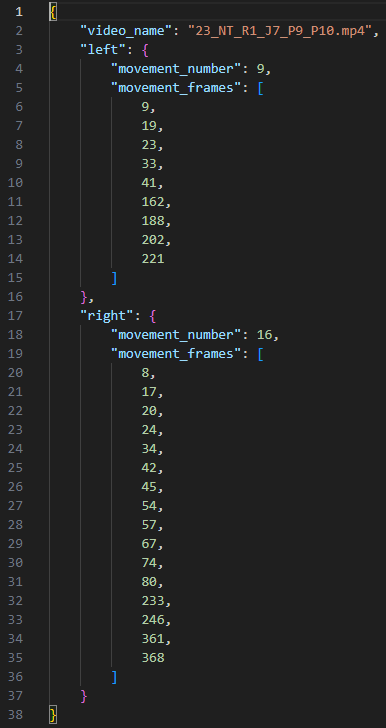
\includegraphics[width=0.32\textwidth]{images/6/6.5/jsonFormat.png}
        \caption{Formato de los resultados guardados en \acrshort{json}}
        \label{fig:JSONFormat}
    \end{figure}
\end{itemize}

Si no se selecciona una carpeta con el selector, se guardará por defecto en la carpeta raíz que contenga el módulo principal o el ejecutable.\newline
Para añadir velocidad, se ha asumido que cada nombre de video es único (esto se indica en el manual de la aplicación), esto nos permite que el archivo guardado sea simplemente añadir la extensión al nombre original. 
Por ejemplo, si tenemos el video \verb|video1.mp4|, los archivos de guardado seran \verb|video1.mp4.csv| y \verb|video1.mp4.json|.

\vspace{1\baselineskip}

Finalmente, para desplegar la aplicación se utilizó la herramienta \texttt{PyInstaller}. Esta herramienta permite crear ejecutables que consiguen encapsular la aplicación de manera que el usuario no necesite 
manejar las dependencias de la aplicación. Además de esto, dentro de la aplicación inserta el intérprete de \texttt{Python}.

Su manera de funcionamiento es, para cada vez que se abra la aplicación, crear un entorno virtual. Y se puede crear un ejecutable creando:
\begin{itemize}
    \item Un ejecutable: contiene todo dentro, por lo tanto también realiza compresión. Suele pesar mucho menos, pero tarda en abrirse, ya que crea en una carpeta temporal del usuario el entorno de \texttt{Python}.
    \item Una carpeta con un ejecutable dentro: funciona de la misma manera que lo anterior, pero las dependencias vienen ya descomprimidas, por lo tanto no le hace falta crear una carpeta temporal y se abre mucho 
    más rápido, sin embargo pesa casi el doble habitualmente.
\end{itemize}

En el caso se han creado las dos versiones, con los siguientes comandos, el primero para crear un ejecutable completo, y el segundo para una carpeta (cambiando --onefile por --onedir):
\begin{lstlisting}[language=bash,breaklines=true]
    pyinstaller --onefile --add-data="C:/Users/Diego/Documents/Codigo/TFG2024/.venv/Lib/site-packages/ultralytics":"ultralytics/" --add-binary="C:/Users/Diego/Documents/Codigo/TFG2024/.venv/Lib/site-packages/openvino/libs":"." --hidden-import openvino --collect-submodules openvino --collect-binaries openvino --collect-data openvino --hidden-import onnx --hidden-import onnxruntime  .\main.py
\end{lstlisting}

\begin{lstlisting}[language=bash,breaklines=true]
    pyinstaller --onedir --add-data="C:/Users/Diego/Documents/Codigo/TFG2024/.venv/Lib/site-packages/ultralytics":"ultralytics/" --add-binary="C:/Users/Diego/Documents/Codigo/TFG2024/.venv/Lib/site-packages/openvino/libs":"." --hidden-import openvino --collect-submodules openvino --collect-binaries openvino --collect-data openvino --hidden-import onnx --hidden-import onnxruntime  .\main.py
\end{lstlisting}

Ambas instrucciones cargan los runtimes necesarios (como el de \texttt{CUDA}, \texttt{ONNX} y \texttt{OpenVino}) para que la aplicación pueda aprovechar al máximo el \texttt{HardWare} y detectar cuál formato de 
modelo de red neuronal utilizar.